\documentclass[a4paper,12pt]{article}
\usepackage[utf8]{inputenc}

\usepackage{amssymb,amsfonts,amsmath,mathtext,geometry,cite,enumerate}
\geometry{left=2cm} \geometry{right=2cm}
\geometry{top=2cm} \geometry{bottom=3cm}

\usepackage[dvips]{graphicx}
\usepackage{wrapfig}

\title{A note about tomography reconstruction}
\author{Mike Konnik}

\begin{document}
\maketitle

The setup for the tomography experiment consists of 3 NGS (simple constellation, equal distance on a circle), 2 atmospheric layers, 1 DM and 1 WFS.  

\begin{wrapfigure}[16]{r}{0.3\linewidth} 
\vspace{-5ex}
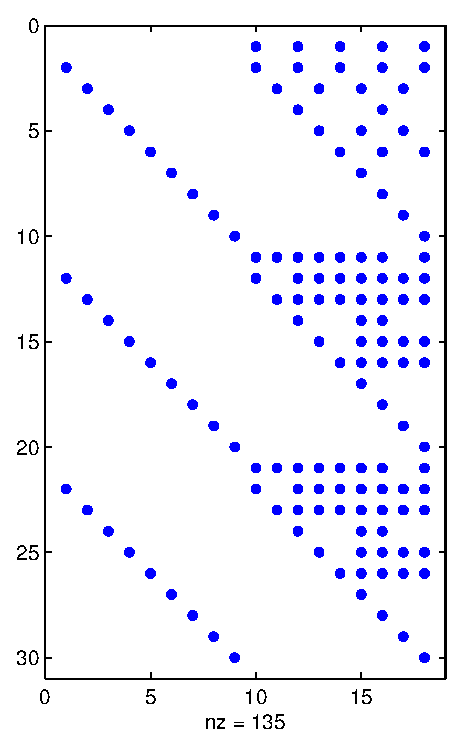
\includegraphics[width=1\linewidth]{Projection_Matrix_spy}
\caption{Typical structure of the projection matrix $P_\alpha$: 10 Zernike modes, $N_\alpha$=3 Gs, and $N_L = 2$ atm layers.}
\label{fig:Projection_Matrix_spy}
\end{wrapfigure}     We have: 

\begin{enumerate}
 \item  $N_z$ is the number of Zernike polynomials,
 \item  $N_s$ is the number of measurements (of slopes), 
 \item $N_L$ is the number of thin atmospheric layers of turbulence, 
 \item $N_\alpha$ is the number of guidestar directions. 
 \item $N_\beta$ is the number of science objects directions. 
\end{enumerate}

Assume a multi-layer atmosphere with $N_L$ thin layers located at altitudes $h_j$ with the phase coefficients $\varphi = [\varphi_0^T \dots \varphi_{N_L}^T ]^T$.  That is, we have:

\begin{enumerate}
 \item  $\phi$ is the phase in the pupil,
 \item  $\varphi$ is the turbulent phase in atmospheric layers
\end{enumerate}

Consider the forward model to represent the relationships between the slopes $S_\alpha = \left[ \begin{array}{c} s_x \\ s_y \end{array} \right]$ and the phase on the telescope pupil $\phi_\alpha$ as:

\begin{equation}
 S_\alpha =  \Gamma  P_\alpha \phi_\alpha + \eta_\alpha
\end{equation}
where $\alpha$ is the direction of the guidestar, $\eta$ is the measurement noise. Here $S_\alpha$ is a column vector of $N_\alpha \times N_s$ measurements of slopes, gradient operator $\Gamma = diag \{ \Gamma_1 \dots \Gamma_{N_\alpha} \}$ (also called $D_z$ in the MATLAB code) of size $[N_\alpha N_s \times N_\alpha N_z ]$.

The phase in the pupil plane (aperture-plane) $\phi_\alpha$ can be related to the phase in the atmospheric layer via projection matrix $P_\alpha$ as $\phi_\alpha =P_\alpha \varphi $. The typical structure of the matrix $P_\alpha $ is shown in Fig.~\ref{fig:Projection_Matrix_spy}



\section{Projection matrix}
The projection matrix $P_\alpha$ will depend on the displacement of the area in telescope's pupil coordinates. Since the atmospheric layer is projected, the projection will contain other modes that have to be accounted. The further the displacement, the more off-diagonal elements we are going to see. We project the displaced atmospheric turbulence patch at the layer $k_L$ that is located at the altitude $h_L$ using the \textbf{TransformC} method.


\subsection{Mathematical background}
The problem here is to find the projection matrix to project the Zernike modes of the atmospheric layers onto the meta-pupil. Consider:
\begin{enumerate}
 \item  $\theta$ is the  zenith angle,
 \item  $\alpha$ is the azimuth angle,
\end{enumerate}

\begin{wrapfigure}[16]{r}{0.4\linewidth} 
\vspace{-12ex}
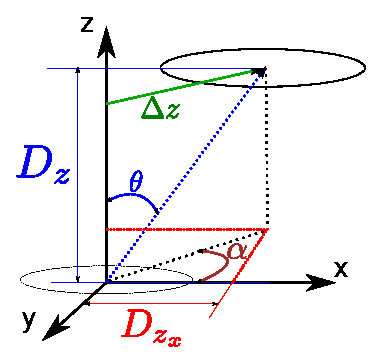
\includegraphics[width=1\linewidth]{layer_above_and_below}
\label{fig:layer_above_and_below}
\end{wrapfigure} as shown in Fig.~\ref{fig:layer_above_and_below}, then in the pupil plane we have the following displacements: 
$$[\delta z_x, \delta z_y] = D_z \tan \theta \,\, [\cos \alpha, \sin \alpha ].$$

Then we have to norm the displacements on the telescope's diameter: 

$$[\delta z'_x, \delta z'_y] = [\delta z_x, \delta z_y] *2 / D_{tel}(h_L),$$

 where $D_{tel}(h_L)$ is the diameter of the telescope at the altitude $h_L$:

$$D_{tel}(h_L) = D_{tel}(0) + 2 h_L \tan(\gamma_{FOV} /2)$$

where $\gamma_{FOV}$ is the field of view (FOV) of the telescope. The \textbf{TransformC} requires a scaling parameter, which is simply $\kappa = \frac{ D_{tel}(h_L)  }{   D_{tel}(0)  }$. 

Then we use either \textbf{smallFootprintExpansion} method (slow) or \textbf{AnalyticalSmallFootprintExpansion} (fast) to get the projection matrix $P_\alpha$.


\subsection{Tomography projection matrices}
We calculate the following projection matrices:
\begin{enumerate}
 \item $P_{DM}$ is the projection for DMs at different DM's conjugation altitudes ($h^j_{DM}$);

 \item $P_{\alpha}$ (also known as $P_{Atm}$)  is the projection of guidestars (sources) onto atmospheric layers at different turbulence altitudes $h^j_{L}$ in the directions $\alpha$ of the guidestars;

 \item $P_{\beta}$ (also known as $P_{Sci}$) is the projection of science objects (sources) onto atmospheric layers at different turbulence altitudes $h^j_{L}$ in the direction$\beta$ of the science objects.
\end{enumerate}

Once again, we have two types of directions:

\begin{enumerate}
 \item guidestar directions $\alpha$,
 \item science directions $\beta$.
\end{enumerate}

Usually, those directions are different, i.e.,  $\alpha \neq  \beta$.





\section{NGS Tomography}
After computing the projection matrices  $P_{\alpha}$ and $P_{\beta}$, we compute the covariance matrices and the reconstruction matrix. As before, $S_\alpha = \Gamma P_\alpha \varphi  + \eta_\alpha $. Therefore, we can find the estimation of the phase as:

$$\hat{\varphi} = [\Gamma P_\alpha ]^{\dagger} S_\alpha $$

Another way is to use minimum-variance (MV) reconstruction and obtain the aperture-plane phase estimate $\hat{\phi}_\beta$ in the $\beta$ science directions as:

$$\hat{\phi}_\beta = \frac{ P_\beta <\varphi \varphi^T> P_\alpha^T \Gamma^T }{ \Gamma P_\alpha  <\varphi \varphi^T> P_\alpha^T \Gamma^T + <\eta \eta^T > }  S_\alpha $$

where $\phi_\beta$ is a $[N_\beta N_z \times 1]$ vector of aperture-plane phase coefficients from the decomposition of the wavefront in all the $N_\beta$ science directions. Here we denote the phase covariance:

\begin{equation}
\Sigma_\phi = <\varphi \varphi^T>,
\end{equation}
which is usually computed theoretically via \textbf{phaseStats.zernikeCovariance} function between the layers of the atmospheric turbulence, and the noise covariance (usually in Zernike modal form) $\Sigma_\eta =  <\eta \eta^T > $.

The cross-correlation matrix of Zernike coefficients from the modes of the atmosphere object for each atmospheric layer $\Sigma_\phi$ is then projected on the directions of guidestars $\alpha$ and science objects $\beta$:

\begin{enumerate}
 \item projection on the guidestars directions $\alpha$:  $\Sigma_{\alpha} = P_{\alpha}  \Sigma_\phi  P_{\alpha}^T$, also expressed $\Sigma_{\alpha} = <\phi_\alpha \phi_\alpha^T>$;
 \item projection on the science objects directions $\beta$:  $\Sigma_{\beta \alpha} = P_{\beta}  \Sigma_\phi  P_{\alpha}^T$, or $\Sigma_{\beta \alpha} = <\phi_\beta \phi_\alpha^T>$;
\end{enumerate}

Then we compute a minimum variance (or static MMSE) reconstruction:

$$R_{mv} = \frac{\Sigma_{\beta \alpha} D_{z.ast}^T  }{ D_{z.ast} \Sigma_\alpha  D_{z.ast}^T  + C_{z.ast}}$$
of size $[nSci \times nGs]$, where  $D_{z.ast} = diag \{ Z_{c.1} \dots Z_{c.NGS} \}$ is the block-diagonal matrix of Zernike coefficients for all NGSes, and $C_{z.ast} = diag \{ \Sigma_{wfs.1} \dots \Sigma_{wfs.NGS} \}$ where $\Sigma_{wfs.i} = Z_{c.i} Z_{c.i}^T$ is a covariance matrix of Zernike modes for slopes at each NGS.

One can compare the initial Zernike modes covariance and the projected one to ensure the projection is performed correctly:

$$trace (\Sigma_z) - trace(\underbrace{P_\alpha \Sigma_{\phi_z}P_\alpha^T}_{\Sigma_\alpha}) \approx 0$$

That is, the projected covariance and the initial one must be very close. 


\subsection{MMSE and Covariance estimation}
We need to estimate the covariance matrices, and can estimate the phase via MMSE as $\bar{S_\alpha} =  \Gamma P_\alpha  \bar{\varphi} + \eta_\alpha $. The phase estimation via MMSE can be done as:

\begin{equation}\label{eq:LMMSEreconstructor}
\bar{\varphi} = \Sigma_{\varphi s}  \Sigma_{s s}^{-1} \bar{S_\alpha} 
\end{equation} 


where the covariance matrices are:: 

$$\Sigma_{s s} = <(\Gamma P_\alpha  \varphi + \eta)(\Gamma P_\alpha   \varphi + \eta)^T> = \Gamma P_\alpha  < \varphi \varphi^T> P_\alpha ^T \Gamma^T + \eta \eta^T  = \Gamma P_\alpha  \Sigma_\varphi   P_\alpha ^T \Gamma^T + \Sigma_\eta $$ 

 and   

$$\Sigma_{\varphi s} = <(\varphi)(\Gamma P_\alpha   \varphi + \eta)^T> = < \varphi \varphi^T> P_\alpha^T \Gamma^T  = \Sigma_\varphi P_\alpha^T \Gamma^T.$$

When the spatial covariance of phase $\Sigma_{\varphi}$ and spatial covariance of noise $\Sigma_\eta$ are known, the minimum variance reconstructor can be computed as:

$$R_{mmse} = \frac{\Sigma_\varphi D^T}{D \Sigma_\varphi D^T  + \Sigma_w}$$

where $D = D_{z.ast} P_\alpha$, and $D_{z.ast}$ is the calibration matrix for WFS that contains the modal (Zernike) response for all the modes that WFS can register. Once the $R_{mmse}$ matrix is computed, the phase can be estimated as $\hat{\varphi} = R_{mmse} S_\alpha$.

All that has left is to convert the phase into control signals, which can be done using the interaction matrix $\Pi$ and $D_{z.ast}$:

$$S_\alpha = \Pi u  \Rightarrow  u = \Pi^\dagger S_\alpha$$

In our OOMAO simulator, there is a matrix $Z_{2U}$ that contains the interaction matrix, and therefore all we need to convert the estimated phase into control signals is:

\begin{equation}
 u = Z_{2U} P_\beta \hat{\varphi}
\end{equation}

which gives the control signals for the DM and compensates the turbulence in the direction of science objects $\beta$.



\subsection{Optimal control and tomography reconstruction}
Consider state space formulation and the forward model:

$$x_{k+1} = A x_k + \eta_k,$$

where $x_k$ is a \textit{composite} state vector (contains previous phase and vibrations). The slopes can be expressed as $S_k = [\Gamma P_\alpha] x_k + D u_k + v_k$. Assuming we have found the evolution matrix $A = blkdiag\{ A_{1} \dots  A_{N_L}\}$, where $N_L $ is the number of atmospheric layers.

Also, we assume that the driving noise statistics of the forward model is:

\begin{equation}
 \Sigma_n = \Sigma_\varphi - A \Sigma_\varphi A^T
\end{equation} 

The numerical evaluation of the noise covariance matrix $\Sigma_n$ can be challenging, since it may (and usually does) contain small eigenvalues\footnote{This is mainly the problem for the DARE solvers, in which case the numerical solution may fail and some tricks (like diagonal loading) maybe necessary.}.

\subsubsection{LQG control}
The discrete-time LQG regulator minimises the cost function:

\begin{equation}
 J(u) = \sum\limits_{k=0}^{\infty} \left(x^T Q x + u^T R u \right)
\end{equation} 

where the weighting matrices are:

\begin{enumerate}
 \item $R = \Sigma_\eta$, which is a noise covariance estimated from slopes $\Sigma_\eta = s_{wfs} s_{wfs}^T$. Must be full rank.
 \item $Q = \frac{\Sigma_n + \Sigma_n^T}{2}$, since the Q matrix in DARE must be positive definite.
\end{enumerate}

Then we solve the Discrete Algebraic Riccati Equation (DARE) to find the asymptotic Riccati estimation error covariance matrix: $\Sigma_\infty = dare(A,B,Q,R)$, where $B = D_{z.ast} P_\alpha$. This will allow us to gte the asymptotic gain matrix for the phase updates~\cite{correia2015spatio} and LQG control:

\begin{equation}\label{eq:hinftygain}
 H_\infty  = \Sigma_\infty G^T (G\Sigma_\infty G^T + \underbrace{\Sigma_\eta}_{=R} )^{-1}
\end{equation} 
where $G = D_{z.ast} P_\alpha$.

We use the predictive estimation of $\hat{\varphi}$ in form:

\begin{eqnarray}
\varphi_{k|k} = \varphi_{k|k-1} +H_\infty(S_{k, \alpha}  - G \varphi_{k|k-1}) \\
\varphi_{k+1|k} = A \varphi_{k|k} 
\end{eqnarray} 

where $H_{\infty}$ is the LQG gain\footnote{The gain can also be expressed like $H_\infty = \frac{\Sigma_\varphi C_{d.turb}^T}{C_{d.turb} \Sigma_\infty C_{d.turb}^T  + \Sigma_w}$, where $\Sigma_w$ is the noise covariance, $\Sigma_\infty $ is the covariance matrix of estimation error. } from \eqref{eq:hinftygain}. First equation computes the current estimate, and the last one makes a one-step ahead prediction~\cite{correia2015spatio}. 

The control signals can be computed in the direction of the science objects as:

$$u = Z_{2U} P_\beta \varphi_{k+1|k}$$

and applied to the DM.




\section{Laser Guide Star tomography}
Laser Guide Stars use the sodium resonance line $\lambda_{Na} = 589$nm. Laser excitation cause sodium to fluoresce in the mesosphere at around 90 km. \textbf{Due to tubulence-induced jitter in the upward propagation of the laser beam, the position of an LGS is uncertain, and therefore wavefront tilt errors cannot be determined from an LGS WFS}. In an AO tomography context, the tilt indetermination on each LGS WFS translates into an inability to determine both global tip and tilt and field-dependent tilt~\cite{flicker2003tilt}, called tilt-anisoplanatism (TA). TA can be modelled by a combination of quadratic WF aberrations at two or more ranges that produce field-dependent tip-tilt (TT), cancelling out in each LGS WFS, except for tilt, which is not sensed. These modes lead to
plate-scale errors in the final science image.



\subsection{Mathematical background of Split Tomography}
Current generation LGS AO systems~\cite{van2006wm} incorporate a low-order natural guide star (NGS) wavefront sensor (WFS) to measure the tip/tilt (TT) modes of the wavefront that are undetectable using a laser beacon owing its uncertain position~\cite{rigaut1992laser}. Proposed MCAO systems will utilize a few low-order NGS WFSs to measure the TT and tilt anisoplanatism (TA) modes as well~\cite{ellerbroek2002wave}. Since most TA occurs in the three quadratic Zernike modes~\cite{ellerbroek2001methods}, it can be controlled by two DMs and sensed by three low-order NGS WFSs. The benefits of the split tomography approach are:
\begin{enumerate}
 \item  a reduced coupling between the LGS- and NGS-controlled modes, 
 \item a more flexible control of the TT and TA modes, 
 \item a simpler formulation of LGS tomography allowing for algorithms with reduced computational complexity and cost.
\end{enumerate}

The method proposed in~\cite{gilles2008split} is based on two separate control loops driven independently by the LGS and NGS measurements. The NGS control loop uses a noise-weighted least-squares wavefront reconstruction matrix to control the two global TT modes and the three TA modes. The LGS control loop uses an iterative, computationally efficient algorithm providing an approximate solution to minimum-variance tomography, and it controls all modes orthogonal to the five NGS modes. 

Following the DM fitting step, a NGS mode-removal step must be performed to project off the five TT/TA modes from the fitting estimate. Denote~\cite{gilles2008split}:
\begin{enumerate}
 \item  $M$ -  the five-column TT/TA modal matrix spanning the NGS actuator subspace
\item  $G_a = \Gamma^{ngs} H_{dm}^{ngs}$ the DM-to-NGS WFS interaction matrix (mapps DM actuators to geometric NGS WFS). 
\item $G_M = G_aM$ is the \textbf{modal} DM-to-NGS WFS interaction matrix;
\item NGS reconstructor $R = G_M^\dagger$ mapping closed-loop NGS WFS measurements, $s^{ngs}$, to the error in the NGS DM actuator command, is defined as the \textbf{noise-weighted pseudoinverse} of the modal DM-to-NGS WFS interaction matrix $G_M = G_aM$
\end{enumerate}

\begin{equation}
 R = G_M^\dagger = (G_M^T W^{ngs} G_M)^{-1} G_M^T W^{ngs}
\end{equation} 

where $W^{ngs} = (diag (\Sigma_\eta ) )^{-1}$ is the inverse of the diagonal NGS measurement-noise covariance matrix.  Such a reconstructor~\cite{gilles2008split} provides a noise-weighted least-squares fit of the
closed-loop NGS WFS measurements to the gradient of the propagated error in the TT/TA modes along the NGS directions.

Assuming that $G_a$ is an accurate model of the NGS WFSs, the NGS loop reconstructs a
given DM shape into the projection of that shape onto the TT and TA modes defining the columns of the modal matrix $M$. That is, $M R G_a$ is a projection matrix onto the range space of $M$:

\begin{equation}\label{eq:noiseprojectionsplittomo}
R G_a =  M^\dagger = (M^T W_a M )^{-1} M^T W_a 
\end{equation} 

where  $W_a = G_a W^{ngs} G_a$,  $M R G_a = P_a = M M^\dagger$, and $W_a$ is a symmetric weighting matrix in actuator space. Note that the projection matrix $P_a$ is $W_a$ orthogonal; i.e., $P_a^2 = P_a$ and $P_a W_a = W_a P_a$. In the absence of noise the Eq.~\ref{eq:noiseprojectionsplittomo} boils down to:

\begin{equation}\label{eq:noiseprojectionsplittomononoise}
R G_a = M^\dagger 
\end{equation} 

and thus $P_a = M M^\dagger $. Projecting the NGS modes out of the LGS DM actuator vector at the output of the DM fitting step (i.e., applying the operator $I - P_a$):

\begin{equation}
s_{TTremoved} = (I-P_a) s
\end{equation} 

will decouple the NGS loop from the LGS measurements.


\subsection{Implementation details of Split Tomography}
The idea is to remove the Tip-Tilt (TT) modes from the LGS signals and then add the TT from the NGS stars. The TT modes are sensed by a QuadCell and the LGS is captured by a regular SH WFS. Then we calculate the projection matrix for both TT and slopes using Eq.~\ref{eq:noiseprojectionsplittomo}. 

In case of LGS, we use the matrix $P_w = M_{TT} M_{TT}^\dagger$ for the noiseless case. The matrix  $M_{TT}$ of size $2w\times 2$, where $w$ is the number of valid lenslets, is formed as: 

\begin{equation}
 M_{TT} = \left[   \begin{array}{cc}  
1,1,\dots 1, 0, 0, \dots 0 \\
0, 0, \dots 0, \,1,1,\dots, 1 \\
                   \end{array} \right]^T
\end{equation} 

When we account for the noise, the matrix $P_w = M_{TT} (M_{TT}^{\Sigma_\eta})^\dagger$, where $ (M_{TT}^{\Sigma_\eta})^\dagger$ is from  Eq.~\ref{eq:noiseprojectionsplittomo}.

The matrix $P_a$ for removing the TT from DM commands computed similarly; the size of $P_a$ is $2d\times 2$, where $d$ is the number of valid DM actuators. For the noiseless case we have $M_{TT,dm} = \frac{1}{2} F^\dagger Z_{2:3}$, where $F$ is the matrix of DM modes, and $Z_{2:3}$ is the matrix of Zernike modes (only Tip and Tilt).

Define the WFS-to-DM interaction matrix as $G_{D}$ (this is \textit{calibDm.D} matrix in OOMAO). Use a LMMSE for the reconstructor in the form $\bar{\varphi} = \Sigma_{\varphi s}  \Sigma_{s s}^{-1} \bar{S_\alpha}$ from \eqref{eq:LMMSEreconstructor}.


The closed-loop operation proceeds as follows:
\begin{enumerate}
 \item remove TT modes from slopes via $(I - P_w)s$ and remove the TT from the DM commands (added on the previous step from NGS measurements) via $G_D(I - P_a)u$, thus:
$$S_{TTremoved} = (I - P_w)s  - G_D (I - P_a) u$$

\item reconstruct the wavefront using LMMSE from \eqref{eq:LMMSEreconstructor}:

$$\bar{\varphi} = \Sigma_{\varphi s}  \Sigma_{s s}^{-1} S_{TTremoved} $$

\item Now add TT from TT stars, and use PI closed-loop controller for TT-loop:

$$ u_{NGS} = u_{NGS} - k* M_{TT,dm}*mean(QuadCell.slopes,2) ; $$

where $M_{TT,dm} = \frac{1}{2} F^\dagger Z_{2:3}$ and $k$ is the closed-loop gain.

\item Add TT control signals from the TT-loop back to the DM commands:

$$u = F^\dagger S_{TTremoved} -  u_{NGS}$$
\end{enumerate}



% \subsection{Preliminary results and testing}







\bibliographystyle{unsrt}\bibliography{tomo}
\end{document}